The panel for this event application is as shown in \Cref{fig:s3hark0}. 
This application does effective free-field site response analysis of a soil column.
In this panel the user specifies a ground motion at the bottom of the column. 
With soil layer properly defined, the motion at the ground surface will be given at the end of the analysis.
\begin{figure}[!htbp]
  \centering {
    
\includegraphics[width=0.8\textwidth]
    {usage/figures/s3hark0.png} }
  \caption{s$^3$hark}
  \label{fig:s3hark0}
\end{figure}

The UI of s$^3$hark is shown in \Cref{fig:s3hark1}.
There are two graphics shown in the left of the panel. The first one is the soil column graphic, 
which shows a visualization of the soil column.
The second one is the mesh and profile graphic, 
which shows the finite element mesh and profile plots.
On the right of the panel are operation area, soil design table, configure tab, layer property tab and response tab. 


\begin{figure}[!htbp]
  \centering {
    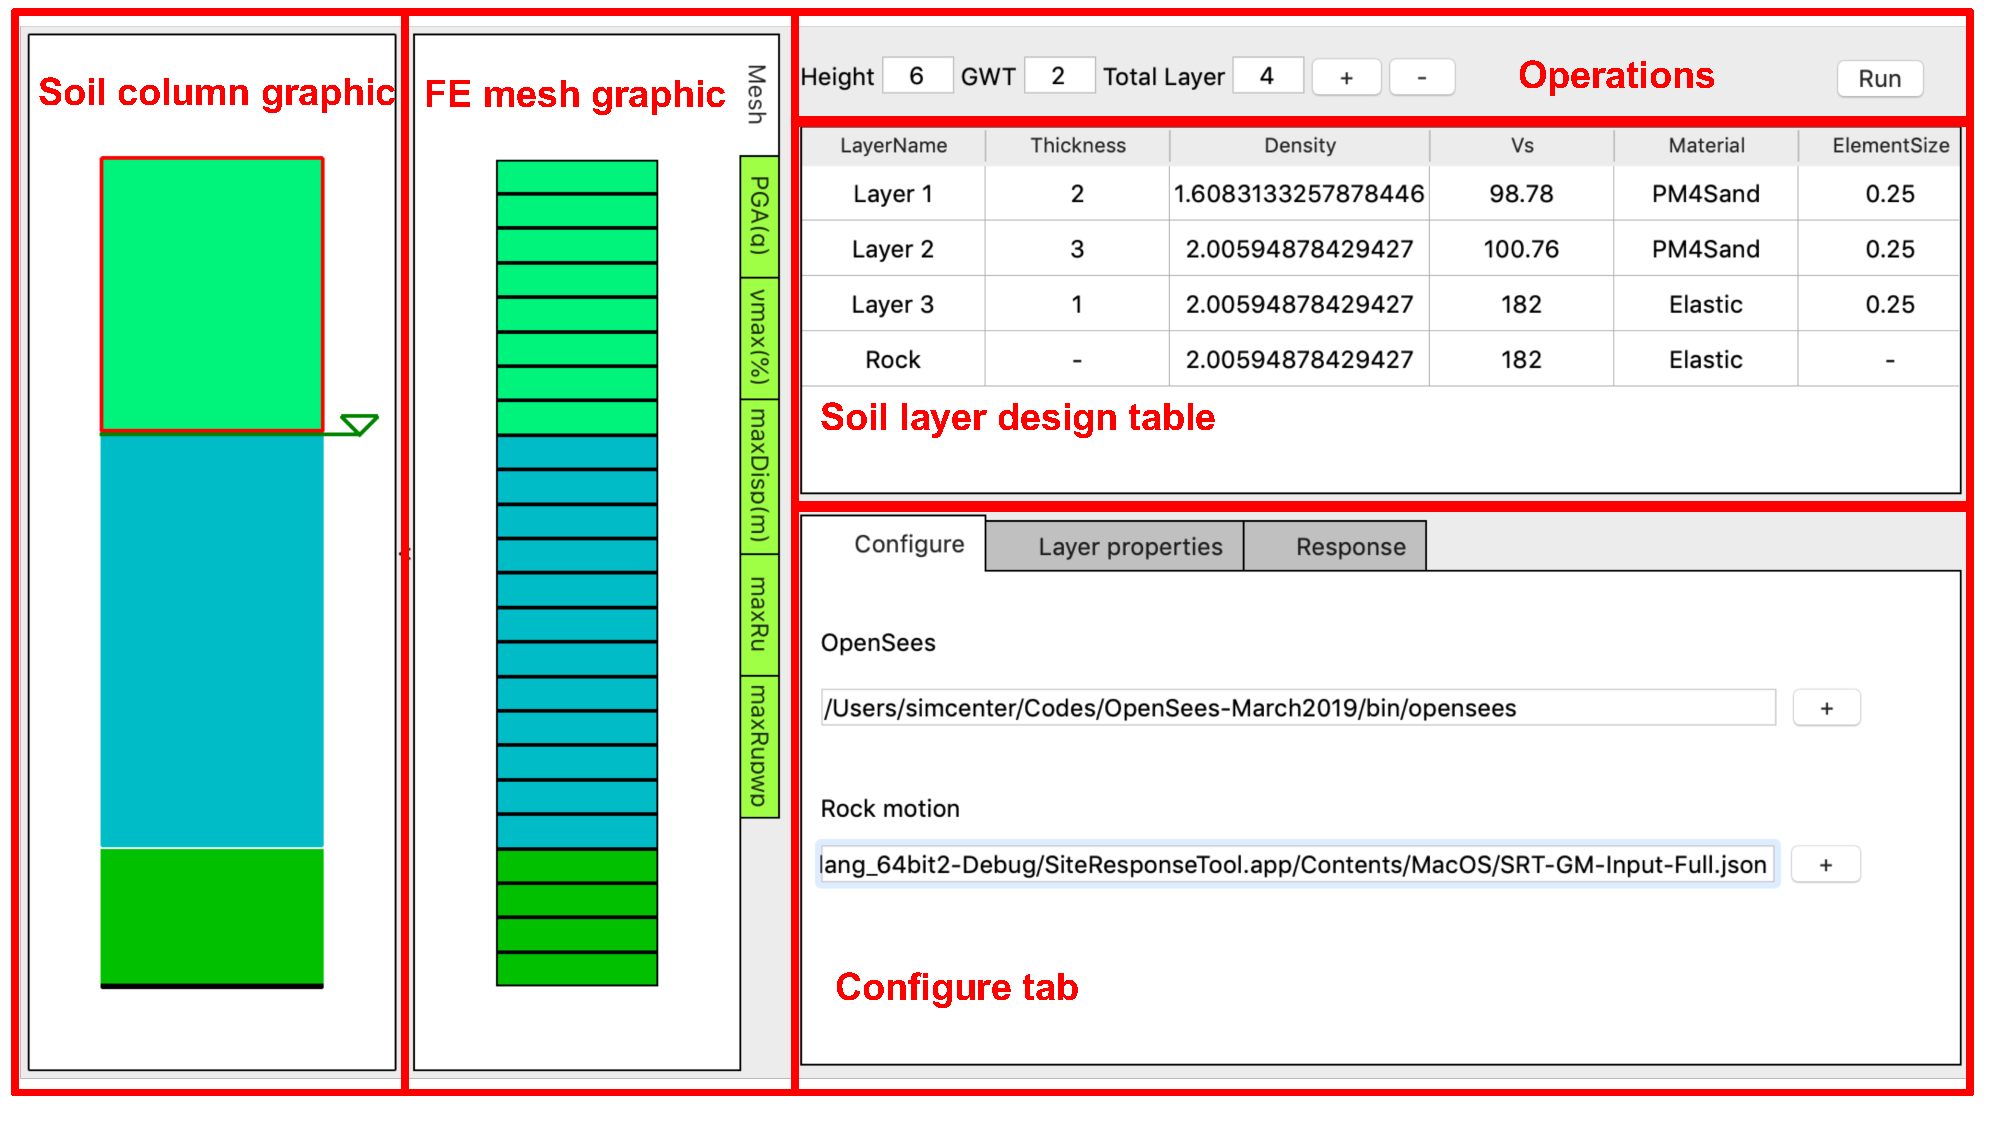
\includegraphics[width=0.8\textwidth]
    {usage/figures/s3hark1.pdf} }
  \caption{s$^3$hark - Panels}
  \label{fig:s3hark1}
\end{figure}

In the operation area as shown in \Cref{fig:s3hark2}, click the plus button to add a layer and the minors button to delete a selected layer. 
Change the ground water table in the GWT input field. 
In the configure tab, path of OpenSees executable and rock motion file need to be specified.
A click on the run button will start the finite element analysis.


\begin{figure}[!htbp]
  \centering {
    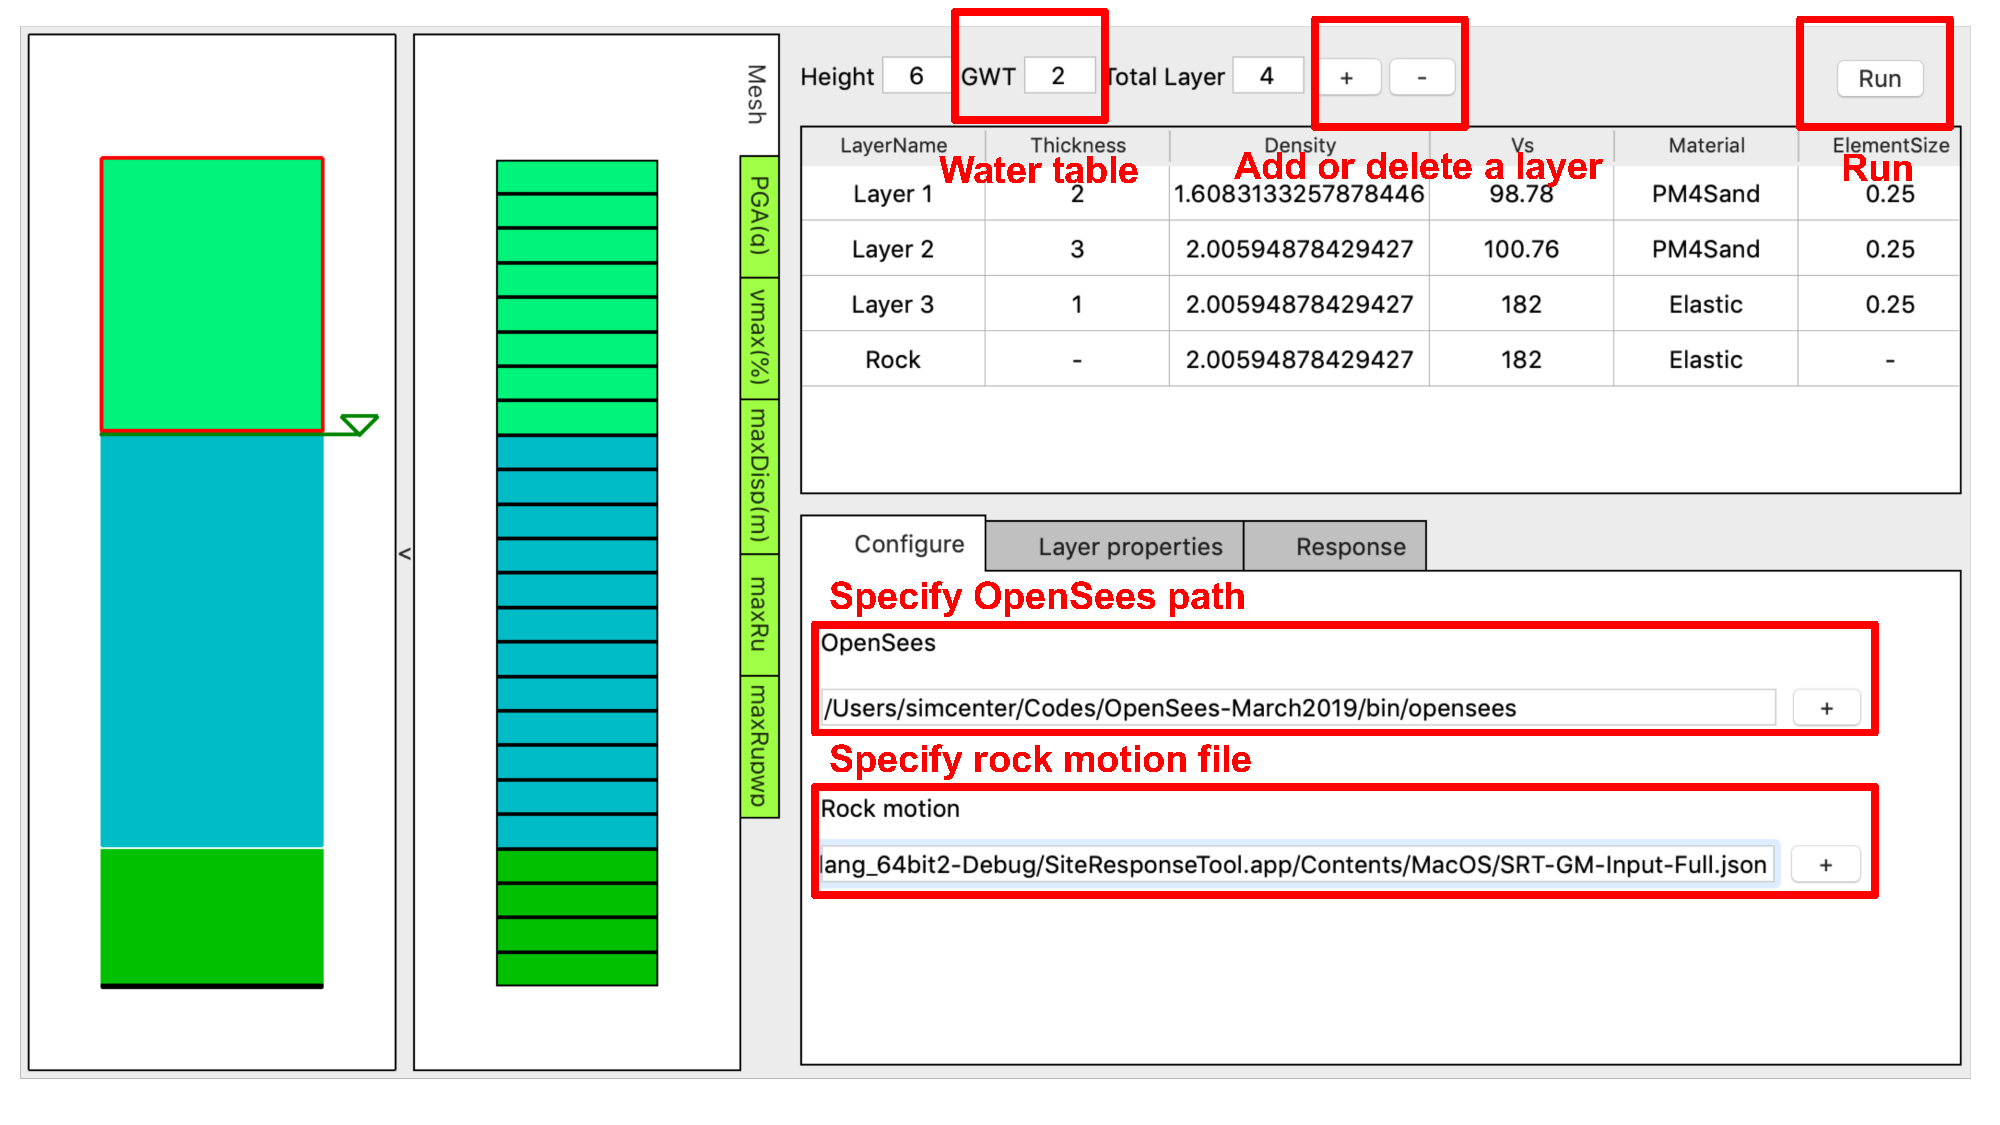
\includegraphics[width=0.8\textwidth]
    {usage/figures/s3hark2.pdf} }
  \caption{s$^3$hark - Configurations and Operations }
  \label{fig:s3hark2}
\end{figure}

Either click on the soil column or the table to select a layer \Cref{fig:s3hark3}. 
When a layer is selected, it will be highlighted in both the soil column graphic and the table. 
Selection of a soil layer will invoke the Layer properties tab, where the user can specify the material properties of this layer.
Double click on a cell of the table will allow the user to change the corresponding value.

\begin{figure}[!htbp]
  \centering {
    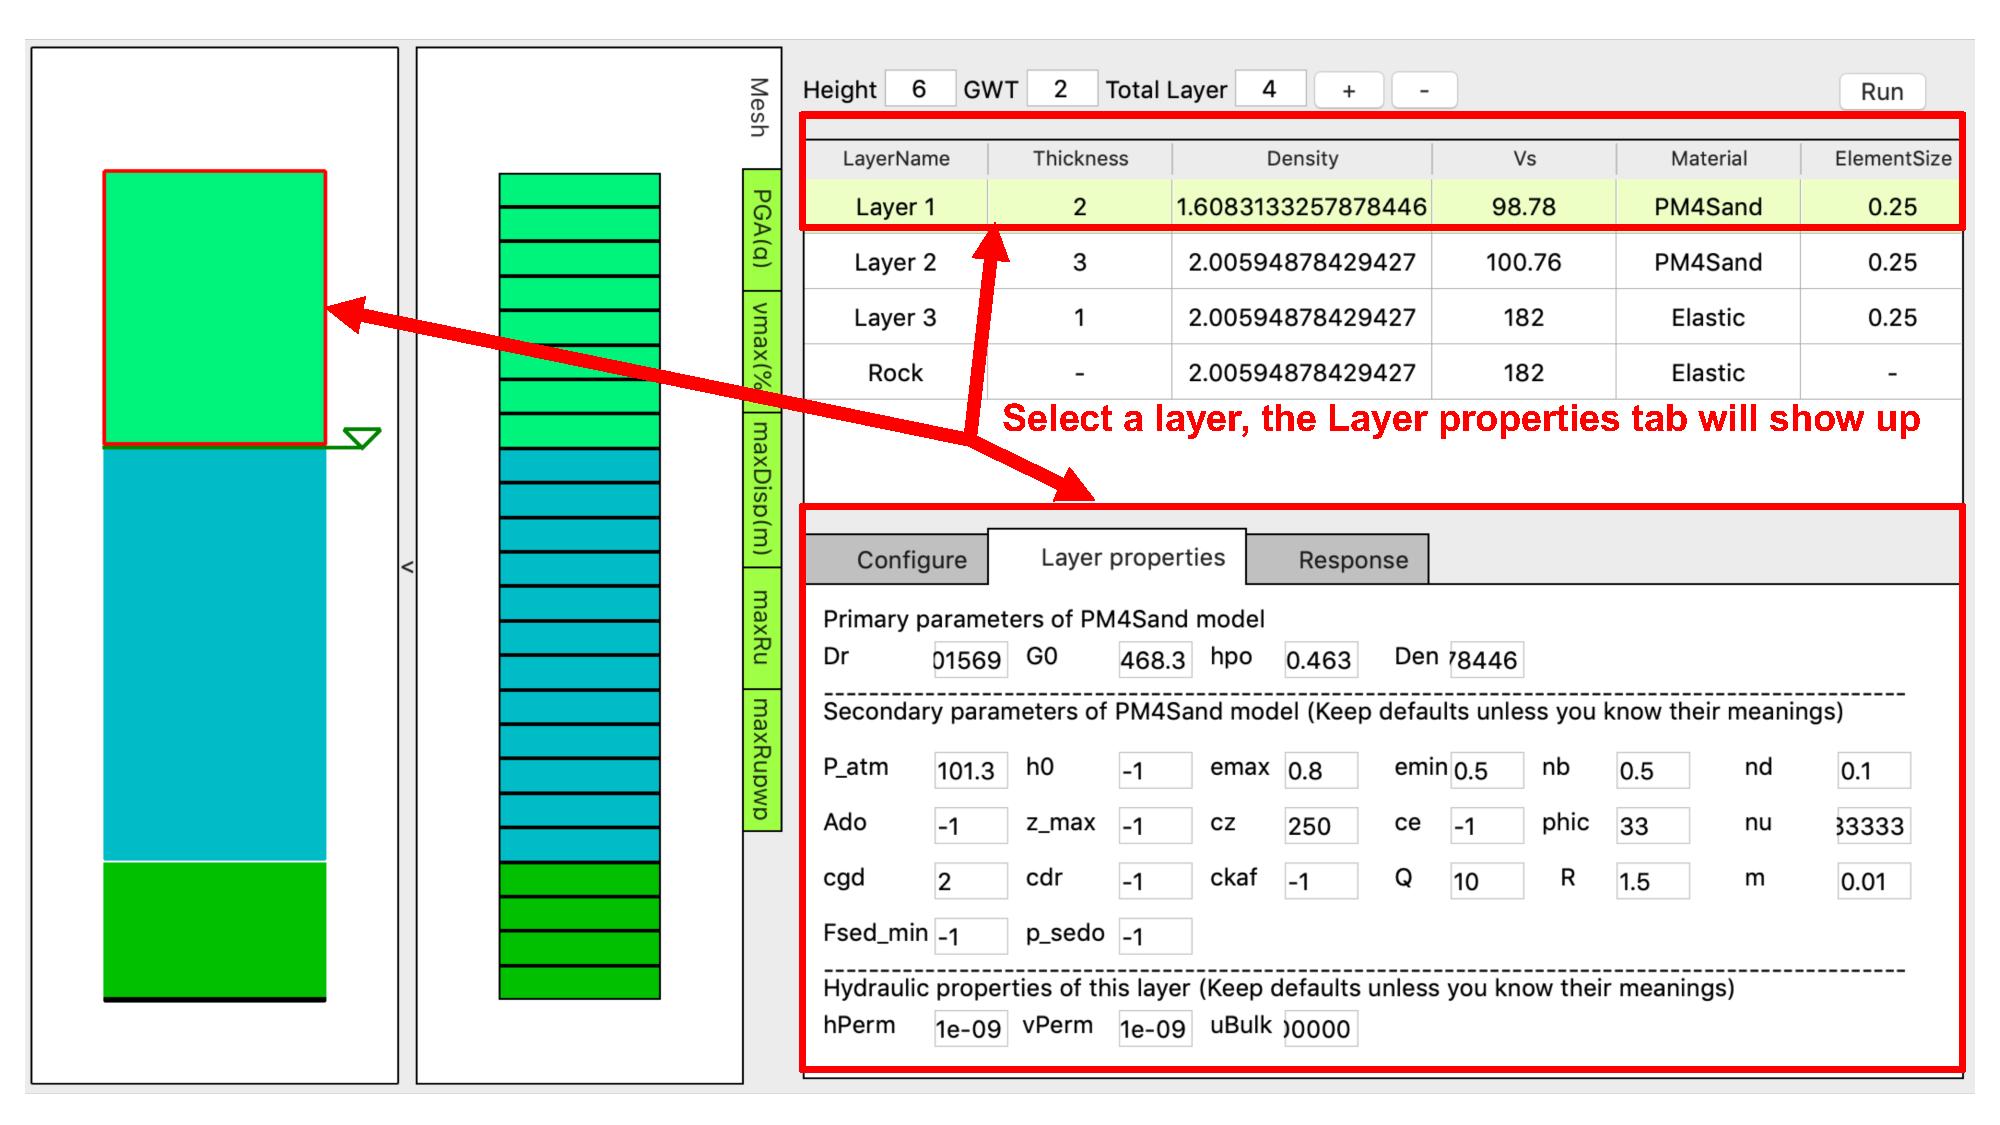
\includegraphics[width=0.8\textwidth]
    {usage/figures/s3hark3.pdf} }
  \caption{s$^3$hark - Layer modification }
  \label{fig:s3hark3}
\end{figure}


Upon the finish of the finite element analysis, the ground motion at the soil surface (\Cref{fig:s3hark4}) will be stored in EE-UQ's input file.
This computed motion will be later applied to the bottom of the building.

\begin{figure}[!htbp]
  \centering {
    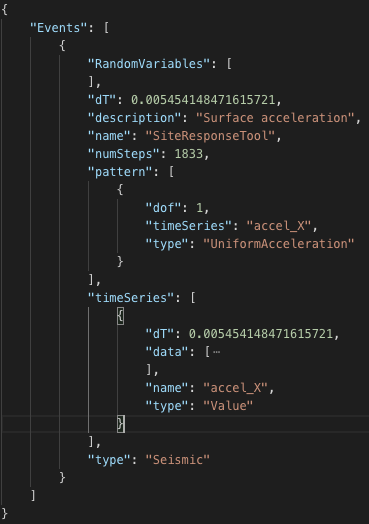
\includegraphics[width=0.4\textwidth]
    {usage/figures/s3hark4.png} }
  \caption{s$^3$hark - Surface motion }
  \label{fig:s3hark4}
\end{figure}
